\clearpage
\section{SOPs}
\label{sec:builder-feature-sops}

This page opens an embedded automation studio that builds flows connecting KayanOS with other accounts and services, starting on a KayanOS event such as a record being created or a form being submitted. Every automation in it works through a KayanOS account connection you choose first. For approval and task workflows inside the organization, “Internal SOPs” is the better fit.

\textbf{Path and who uses it:} “Builder” → “Core” → “SOPs”. Used by those with forms permission who need to connect KayanOS with other systems.

\begin{rcnote}[Example: Horizon]
Horizon wants a message to reach an external tracking sheet whenever a visit request is created. So the system administrator builds an automation that starts when a new record is created in “Visit requests”, then checks the branch before sending the data.
\end{rcnote}

\begin{table}[H]
\centering
\caption{The parts of an automation}
\label{tab:builder-sops-parts}
\begin{tabularx}{\linewidth}{R{3.6cm} Y}
\rcHeaderRow
\thh{Part} & \thh{Meaning}\\
Connection & The KayanOS account the automation acts as, chosen first. Give it only the permissions the work needs.\\
Trigger & The event that starts the automation, such as a record created or updated, or an action on a form or task.\\
Condition & Checks the data before any write, so the automation does not act on records that are not its concern.\\
Actions & What the automation does: create, update or find records, create tasks, send a notification and more.\\
\end{tabularx}
\end{table}

\begin{figure}[H]
\centering
\begin{tikzpicture}[node distance=0.5cm]
\node[stepBox] (a) {Choose the connection};
\node[stepBox,below=of a] (b) {Trigger};
\node[stepBox,below=of b] (c) {Condition before writing};
\node[stepBox,below=of c] (d) {One action at a time};
\draw[flowsTo] (a) -- (b);
\draw[flowsTo] (b) -- (c);
\draw[flowsTo] (c) -- (d);
\end{tikzpicture}
\rclegend
\caption{The order for building an automation}
\label{fig:builder-sops-flow}
\shotnote{The diagram puts the condition before the action, because an automation that writes without checking can change many records in a moment. Test the parts one by one: the trigger alone, then the condition both ways, then each action separately.}
\end{figure}

\subsection{Steps and check}
\begin{enumerate}
\item Open “SOPs”, create a new flow, then choose a KayanOS connection.
\item Choose the trigger and test it with sample data.
\item Add a condition that checks the data, then add the actions one after another, testing each one.
\item Turn the automation on after the tests pass, then review the first real run.
\end{enumerate}

\textbf{Check and recovery:} the run should appear in the automation's history with the expected result. If the page stays empty or shows an error, the automation service may not be available in your organization's environment; on the \en{test2} test environment the page was empty when checked. If an action fails, check the connection's permissions first.

\clearpage
\section{Bots}
\label{sec:builder-feature-bots}

A bot is an assistant with a name and picture that members add to chat, email or calendar. On this page you decide where it can be added, whether it is added automatically, and how it reaches email. What the bot does when messaged or mentioned is built in “Internal SOPs” with triggers such as “On Direct Message to Bot” and “On Mention”.

\textbf{Path and who uses it:} “Builder” → “Core” → “Bots”. Used by those with bots permission.

\begin{rcnote}[Example: Horizon]
The system administrator creates a “Visits assistant” bot and makes it addable to direct chats. When Omar Haddad messages it, an internal SOP starts and replies with the status of his visit request. The bot starts from ①.
\end{rcnote}

\begin{figure}[H]
\centering
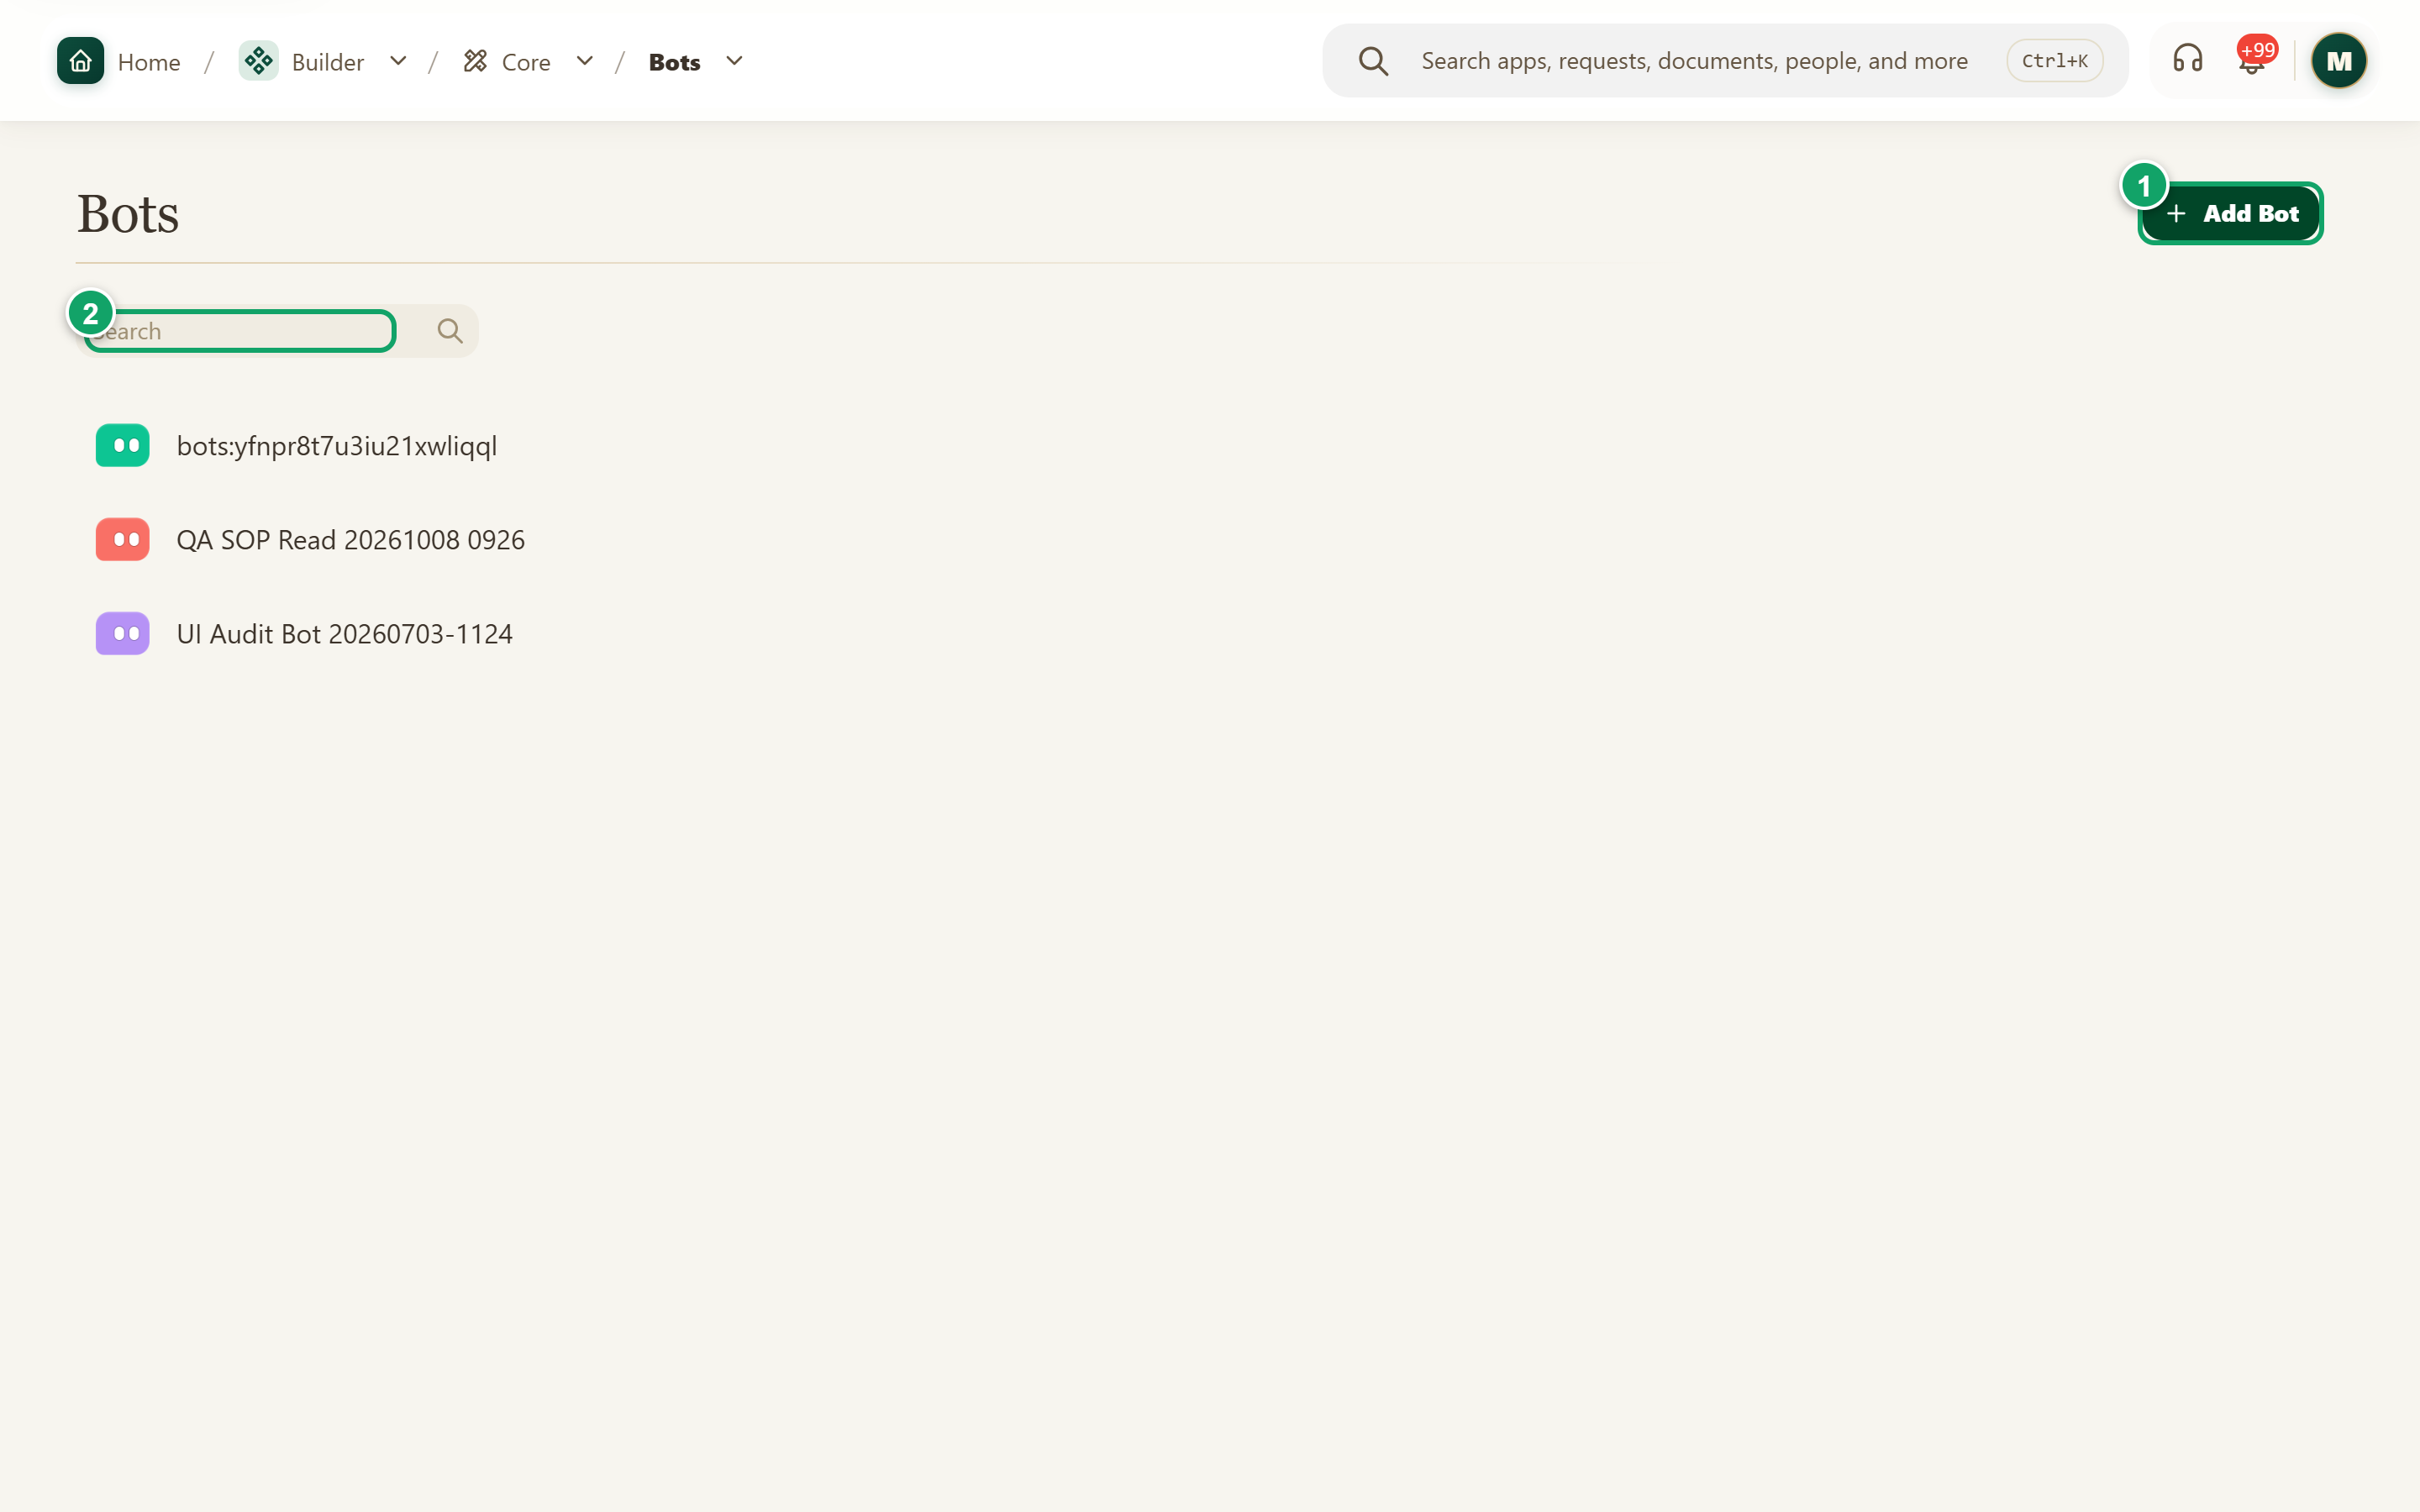
\includegraphics[width=0.95\linewidth,height=0.72\textheight,keepaspectratio]{figures/screens/ch06-bots-en.png}
\caption{The “Bots” page}
\label{fig:builder-bots-screen}
\shotnote{The page lists the organization’s bots, here test bots. ① “Add Bot”: asks only for a name. ② Search: finds a bot by name.}
\end{figure}


\begin{table}[H]
\centering
\caption{Bot settings}
\label{tab:builder-bots-data}
\begin{tabularx}{\linewidth}{R{3.6cm} Y}
\rcHeaderRow
\thh{Section} & \thh{What do you set?}\\
Add Bot & Asks only for the name; the picture is chosen automatically.\\
Chat & Whether it can be added to direct chats or channels, and whether it can be messaged or mentioned.\\
Emails & Whether it is installable in email, can be CCed, and can add internal or external contacts.\\
Calendar & Whether it can be installed in the calendar.\\
Default installation & Whether it is added automatically to chat, email or calendar, and its default email access.\\
\end{tabularx}
\end{table}

\begin{figure}[H]
\centering
\begin{tikzpicture}[node distance=0.5cm]
\node[entity] (bot) {Bot};
\node[entityOpt,below right=0.7cm and 0.3cm of bot] (where) {Where it is added};
\node[entityOpt,below left=0.7cm and 0.3cm of bot] (sop) {Internal SOP that replies};
\draw[dependsOnOpt] (bot.south) -- ++(0,-0.3) -| (where.north);
\draw[dependsOnOpt] (bot.south) -- ++(0,-0.3) -| (sop.north);
\end{tikzpicture}
\rclegend
\caption{The bot's identity and its work}
\label{fig:builder-bots-model}
\shotnote{The figure separates two things: this page sets the bot's identity and where it can be added, while its replies come from an internal SOP that starts when the bot is messaged or mentioned. So a bot does nothing on its own until you connect it to a published SOP.}
\end{figure}

\subsection{Steps and check}
\begin{enumerate}
\item Open “Bots”, press “Add Bot”, write the name and press “Create”.
\item Open the bot, turn on where it can be added in chat, email and calendar, then press “Save”.
\item In “Internal SOPs”, build an SOP that starts “On Direct Message to Bot” and publish it.
\end{enumerate}

\textbf{Check and recovery:} add the bot to a test chat and message it; the SOP should start and appear under “Runs”. If members do not see the option to add it, review the chat settings and save; if the bot does not reply, make sure the SOP is published and not paused.
